\documentclass[aspectratio=169]{beamer}
\usetheme{Madrid}
\usecolortheme{default}
\usepackage{graphicx}
\usepackage{booktabs}
\usepackage{amsmath}

\setbeamertemplate{navigation symbols}{}
\setbeamertemplate{footline}[frame number]

\title{Paraphraser Fingerprinting}
\subtitle{Can We Identify the Rewriter from the Text Alone?}
\author{Boyuan Zhang \and Yange Wang \and Yang-ching Liao}
\institute{Northeastern University, Seattle WA}
\date{}

\begin{document}

% ── Title ──────────────────────────────────────────────────────────────────────
\begin{frame}
  \titlepage
\end{frame}

% ── Problem ────────────────────────────────────────────────────────────────────
\begin{frame}{Research Question}
  \begin{block}{RQ: Paraphraser Fingerprints}
    Do different paraphrasing models leave distinct, detectable traces?\\
    Can we identify the paraphraser from the text alone?
  \end{block}
  \vspace{1em}
  \begin{itemize}
    \item 4 paraphrasers: Llama-3.1-8B, Gemini-2.5-Flash, GPT-5-Nano, DIPPER
    \item Detective (Claude Sonnet 4.6) matches outputs to paraphraser
    \item Auditor (Claude Sonnet 4.6) iteratively crafts adversarial source texts
  \end{itemize}
\end{frame}

% ── Dataset ────────────────────────────────────────────────────────────────────
\begin{frame}{Dataset \& Trial Protocol}
  \textbf{20 trials per run}
  \begin{itemize}
    \item Trial 1 only: hand-crafted text with linguistic traps (grammar, repetition, temporal disorder)
    \item Trials 2--20: Auditor-generated via APE-style iterative refinement
  \end{itemize}
  \vspace{0.8em}
  \textbf{Each trial:}
  \begin{enumerate}
    \item Auditor generates source text
    \item 1 random paraphraser produces 2 outputs; other 3 produce 1 each \textrightarrow\ 5 total
    \item Outputs shuffled
    \item Detective identifies the matching pair
    \item Result fed back to Auditor
  \end{enumerate}
\end{frame}

% ── Experiment Setup (full page) ───────────────────────────────────────────────
{
\setbeamertemplate{footline}{}
\begin{frame}[plain]
  \begin{center}
    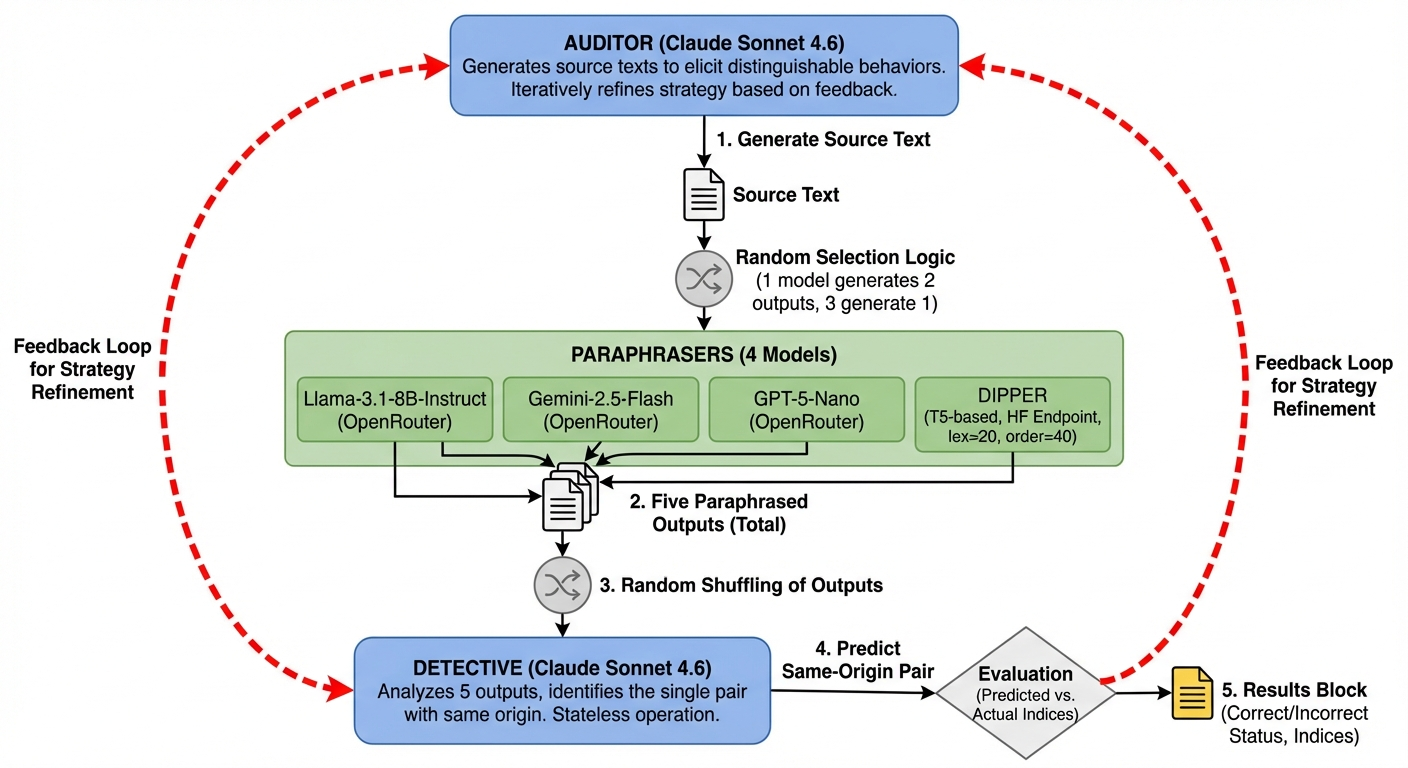
\includegraphics[width=\paperwidth,height=\paperheight,keepaspectratio]{figures/experiment setup.jpeg}
  \end{center}
\end{frame}
}

% ── Aggregate Accuracy ─────────────────────────────────────────────────────────
\begin{frame}{Aggregate Accuracy}
  \begin{columns}
    \begin{column}{0.55\textwidth}
      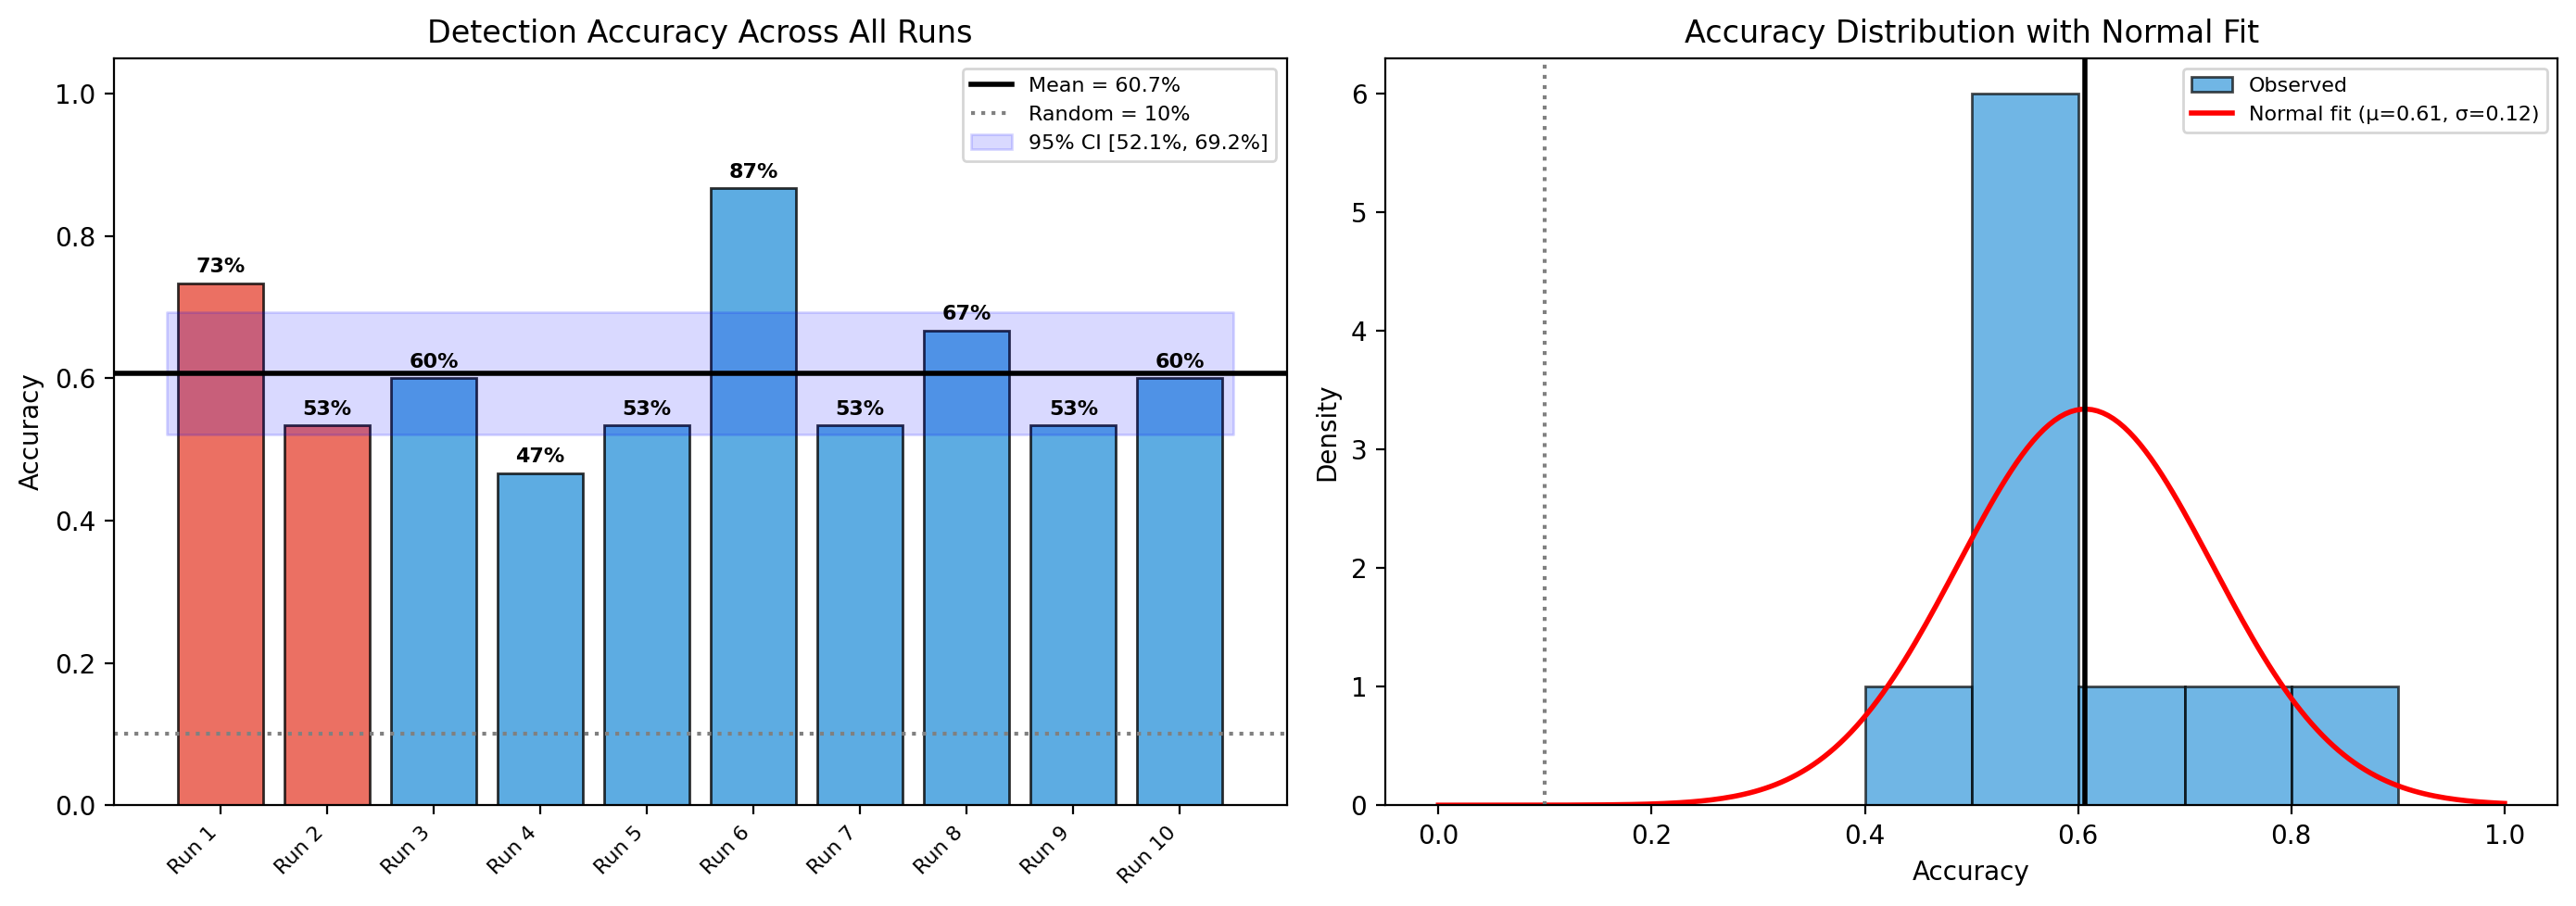
\includegraphics[width=\linewidth]{figures/fig1_accuracy_distribution.png}
    \end{column}
    \begin{column}{0.42\textwidth}
      \begin{itemize}
        \item \textbf{Mean: 60.7\%} across 10 runs (range 47--87\%)
        \item Random baseline: 10\%
        \item Statistically significant: $t(9)=13.41$, $p<0.001$
        \item Detective reliably above chance
      \end{itemize}
    \end{column}
  \end{columns}
\end{frame}

% ── Learning Curve ─────────────────────────────────────────────────────────────
\begin{frame}{Per-Trial Learning Curve}
  \begin{columns}
    \begin{column}{0.58\textwidth}
      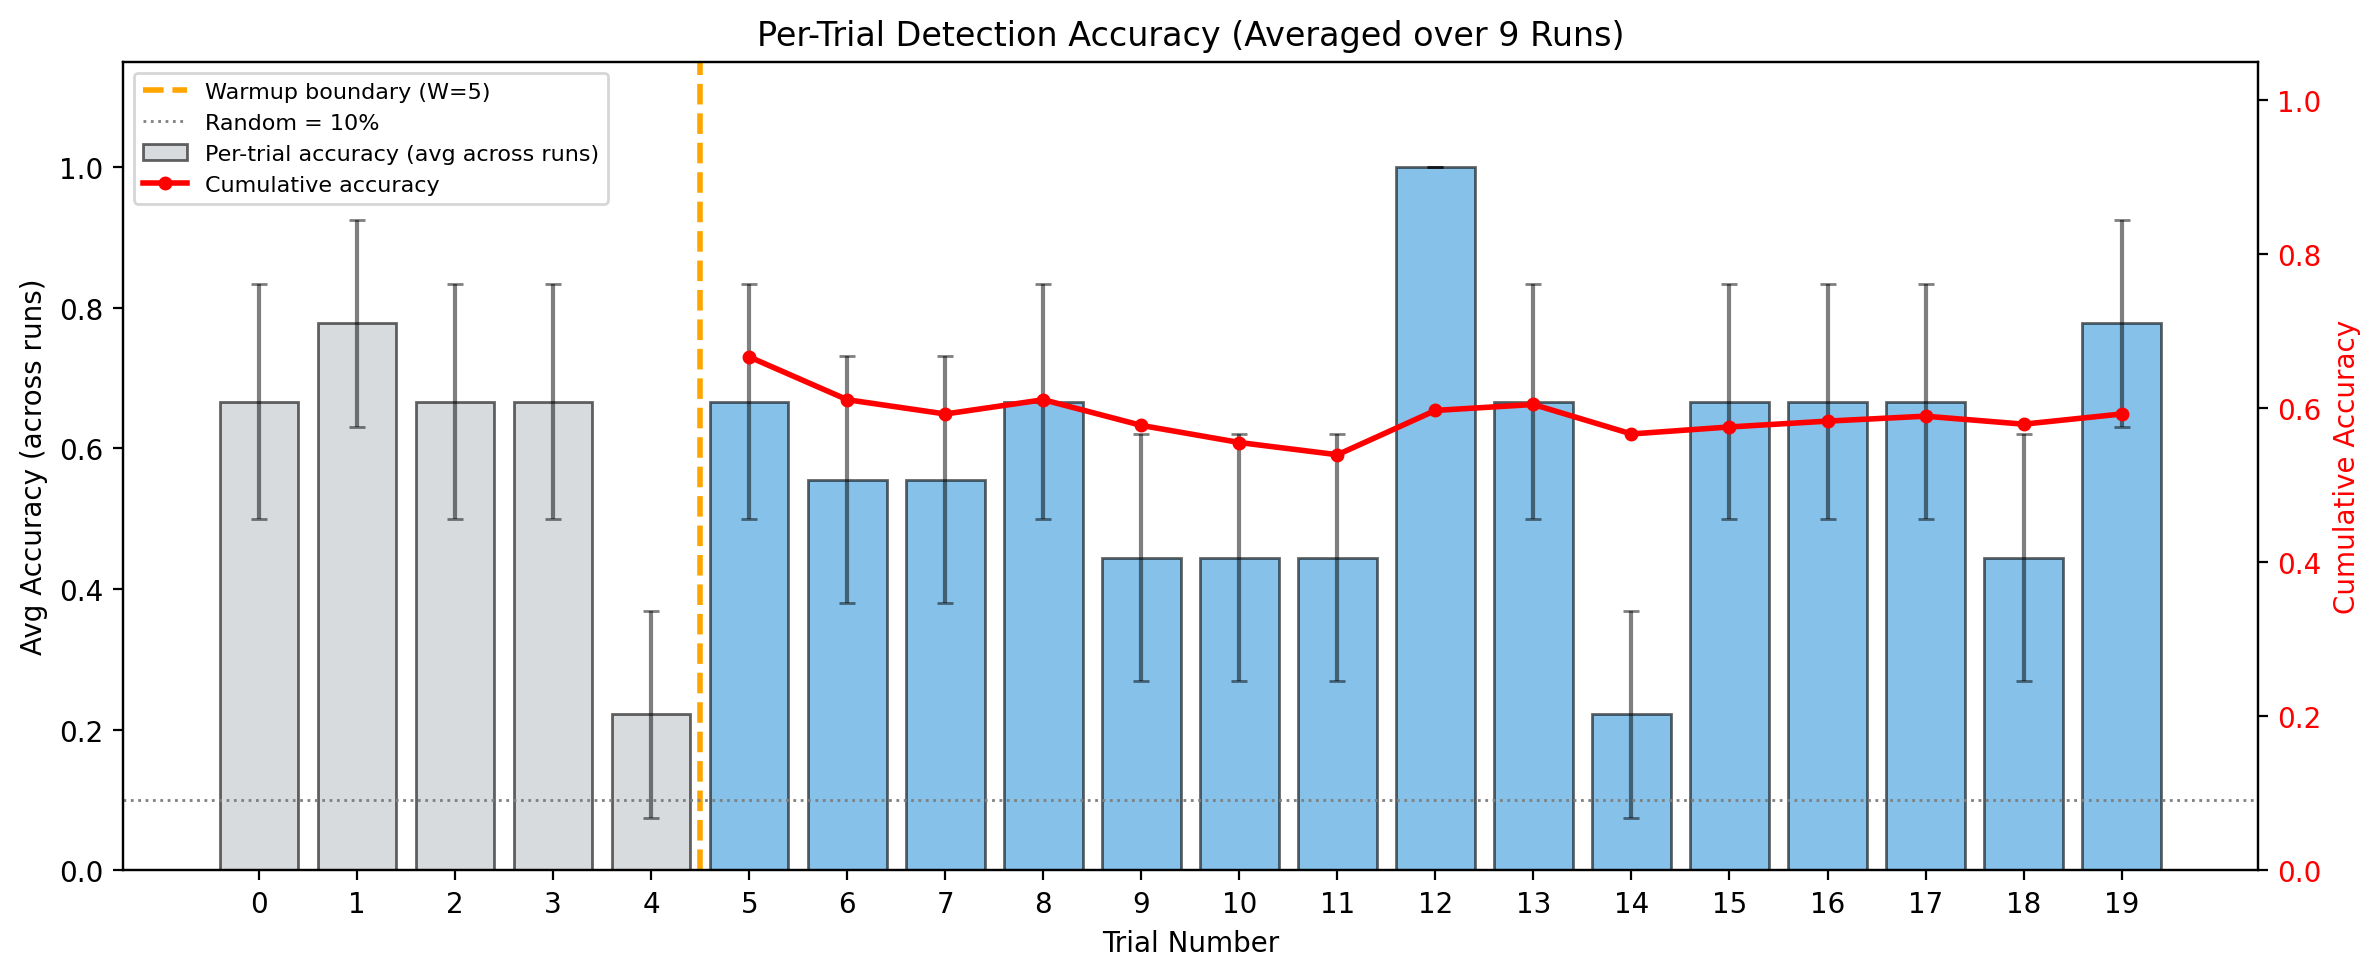
\includegraphics[width=\linewidth]{figures/fig2_per_trial_accuracy_curve.png}
    \end{column}
    \begin{column}{0.38\textwidth}
      \begin{itemize}
        \item Trials 1--5: warm-up
        \item Red curve = cumulative accuracy from trial 5+
        \item Auditor's APE refinement visible in later trials
      \end{itemize}
    \end{column}
  \end{columns}
\end{frame}

% ── Per-Paraphraser Detection ──────────────────────────────────────────────────
\begin{frame}{Per-Paraphraser Detection Rates}
  \begin{columns}
    \begin{column}{0.55\textwidth}
      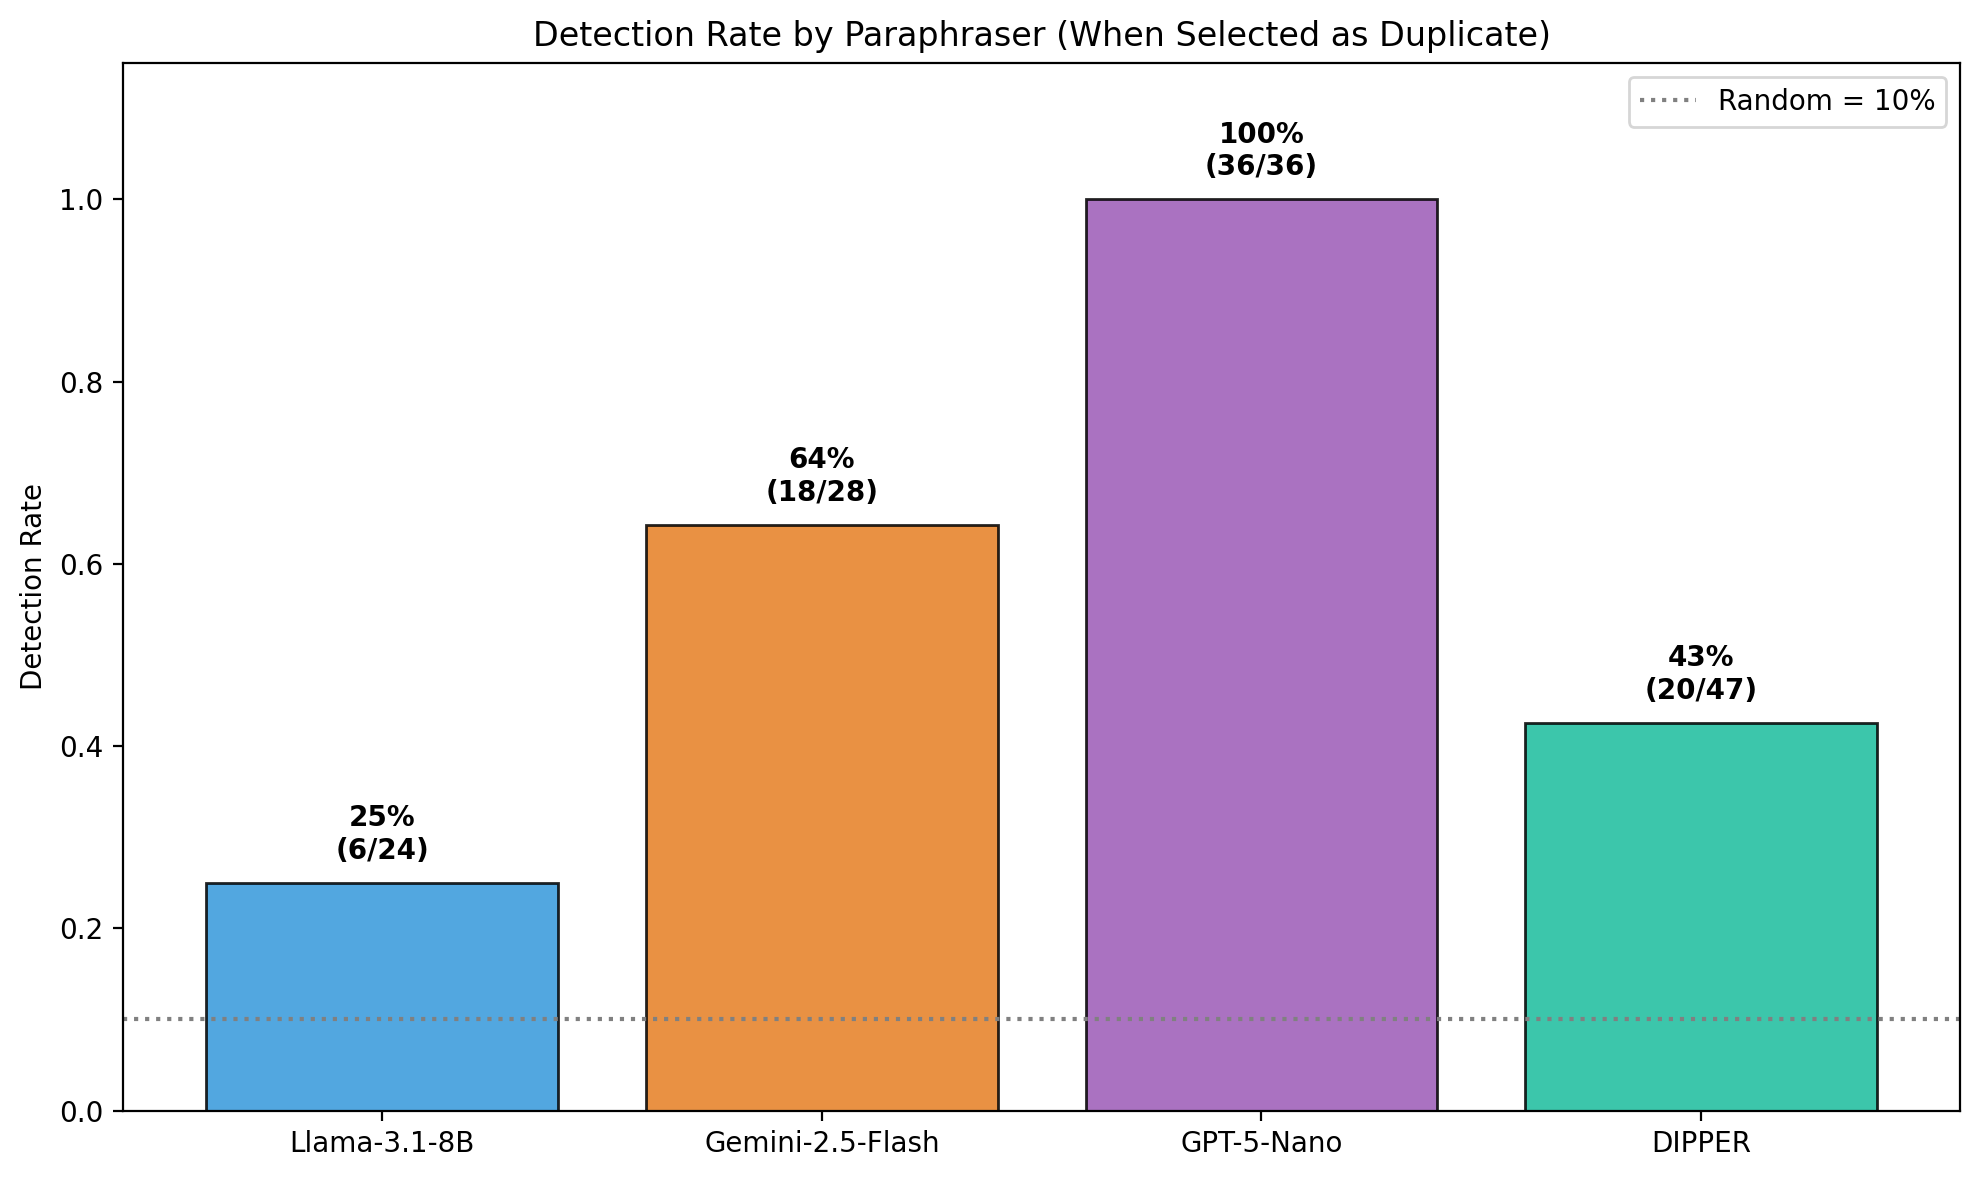
\includegraphics[width=\linewidth]{figures/fig3_paraphraser_detection_rate.png}
    \end{column}
    \begin{column}{0.42\textwidth}
      \begin{itemize}
        \item \textbf{GPT-5-Nano}: \textbf{100\%} (36/36)
        \item \textbf{Gemini-2.5-Flash}: 64.3\% (18/28)
        \item \textbf{DIPPER}: 42.6\% (20/47)
        \item \textbf{Llama-3.1-8B}: 25.0\% (6/24)
      \end{itemize}
      \vspace{0.5em}
      Fingerprint strength varies dramatically across models.
    \end{column}
  \end{columns}
\end{frame}

% ── Confusion Matrix ──────────────────────────────────────────────────────────
\begin{frame}{Confusion Analysis}
  \begin{columns}
    \begin{column}{0.48\textwidth}
      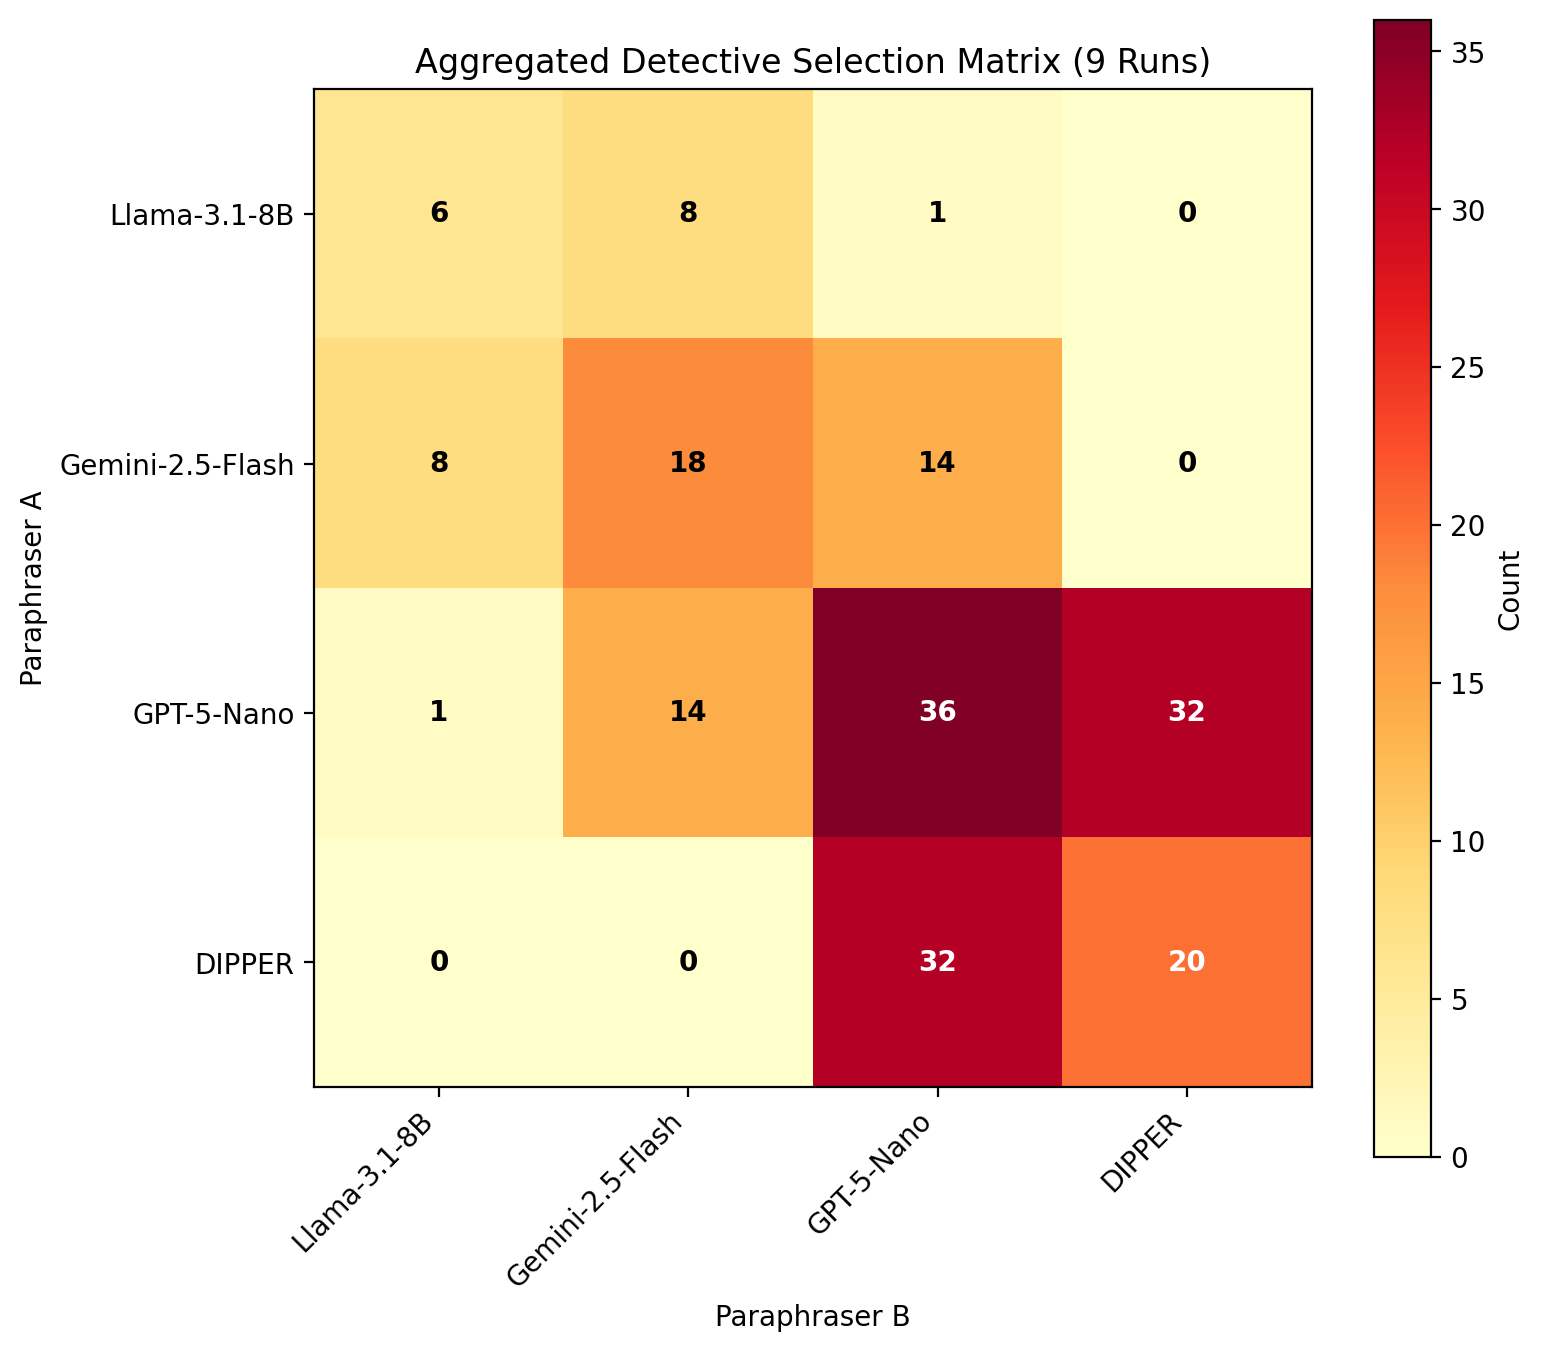
\includegraphics[width=\linewidth]{figures/fig4_confusion_heatmap.png}
    \end{column}
    \begin{column}{0.48\textwidth}
      \begin{itemize}
        \item \textbf{GPT-5-Nano $\leftrightarrow$ DIPPER} (32): most confused pair despite different architectures
        \item Gemini $\leftrightarrow$ GPT-5-Nano (14): moderate LLM-LLM confusion
        \item \textbf{DIPPER $\leftrightarrow$ Llama}: never confused (0)
      \end{itemize}
    \end{column}
  \end{columns}
\end{frame}

% ── Response Length ───────────────────────────────────────────────────────────
\begin{frame}{Response Length as Fingerprint}
  \begin{columns}
    \begin{column}{0.55\textwidth}
      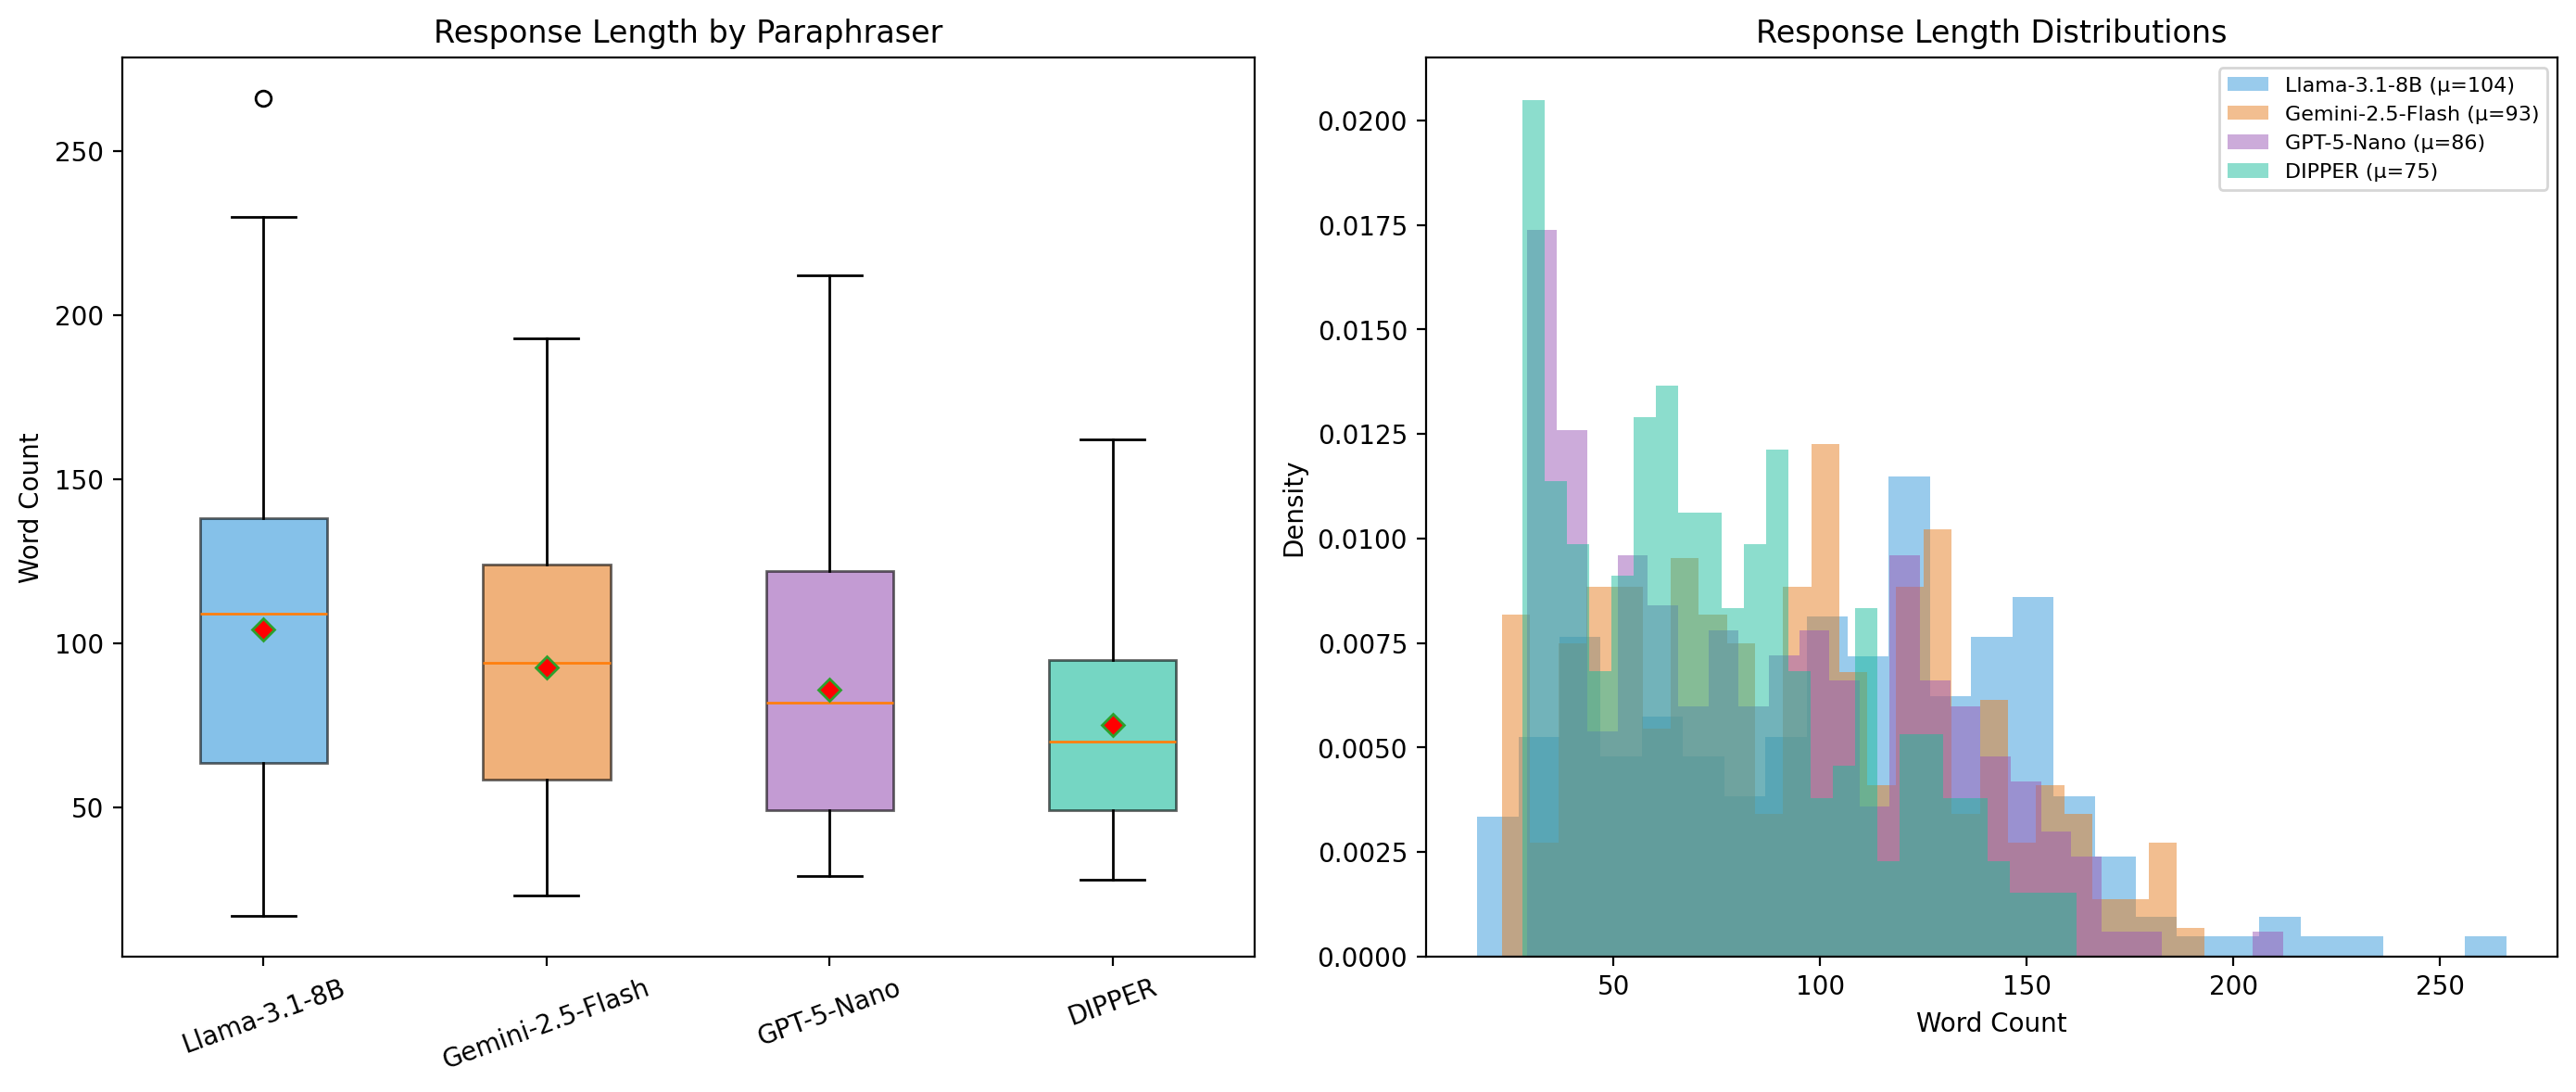
\includegraphics[width=\linewidth]{figures/fig5_response_length.png}
    \end{column}
    \begin{column}{0.42\textwidth}
      \begin{tabular}{lr}
        \toprule
        \textbf{Model} & \textbf{Mean (w)} \\
        \midrule
        Llama-3.1-8B     & 104 \\
        Gemini-2.5-Flash & 93  \\
        GPT-5-Nano       & 86  \\
        DIPPER           & 75  \\
        \bottomrule
      \end{tabular}
      \vspace{0.6em}
      \begin{itemize}
        \item GPT-5-Nano: moderate length but \textbf{strongest fingerprint}
        \item Length alone insufficient---style matters more
      \end{itemize}
    \end{column}
  \end{columns}
\end{frame}

% ── Source Type ───────────────────────────────────────────────────────────────
\begin{frame}{Source Text Type Comparison}
  \begin{columns}
    \begin{column}{0.50\textwidth}
      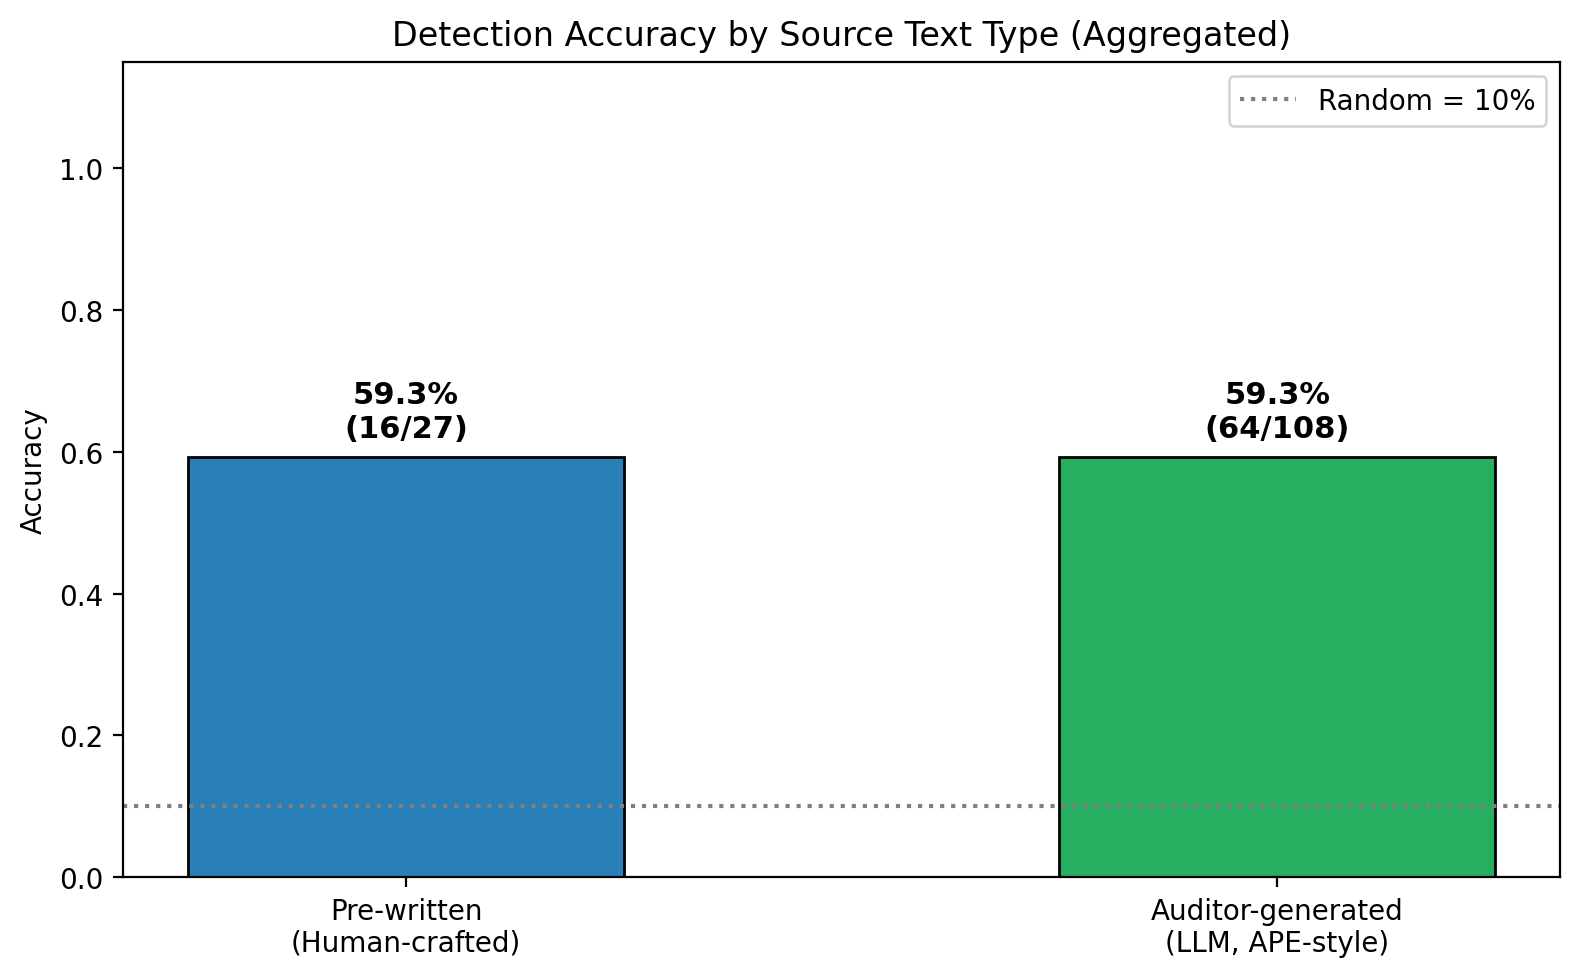
\includegraphics[width=\linewidth]{figures/fig6_source_type_accuracy.png}
    \end{column}
    \begin{column}{0.46\textwidth}
      \begin{itemize}
        \item Human-crafted: \textbf{59.3\%}
        \item Auditor-generated: \textbf{59.3\%}
        \item APE-style refinement matches human-designed traps
        \item Validates automated source generation strategy
      \end{itemize}
    \end{column}
  \end{columns}
\end{frame}

% ── Rationale Analysis ────────────────────────────────────────────────────────
\begin{frame}{Detective Rationale Analysis}
  \begin{columns}
    \begin{column}{0.55\textwidth}
      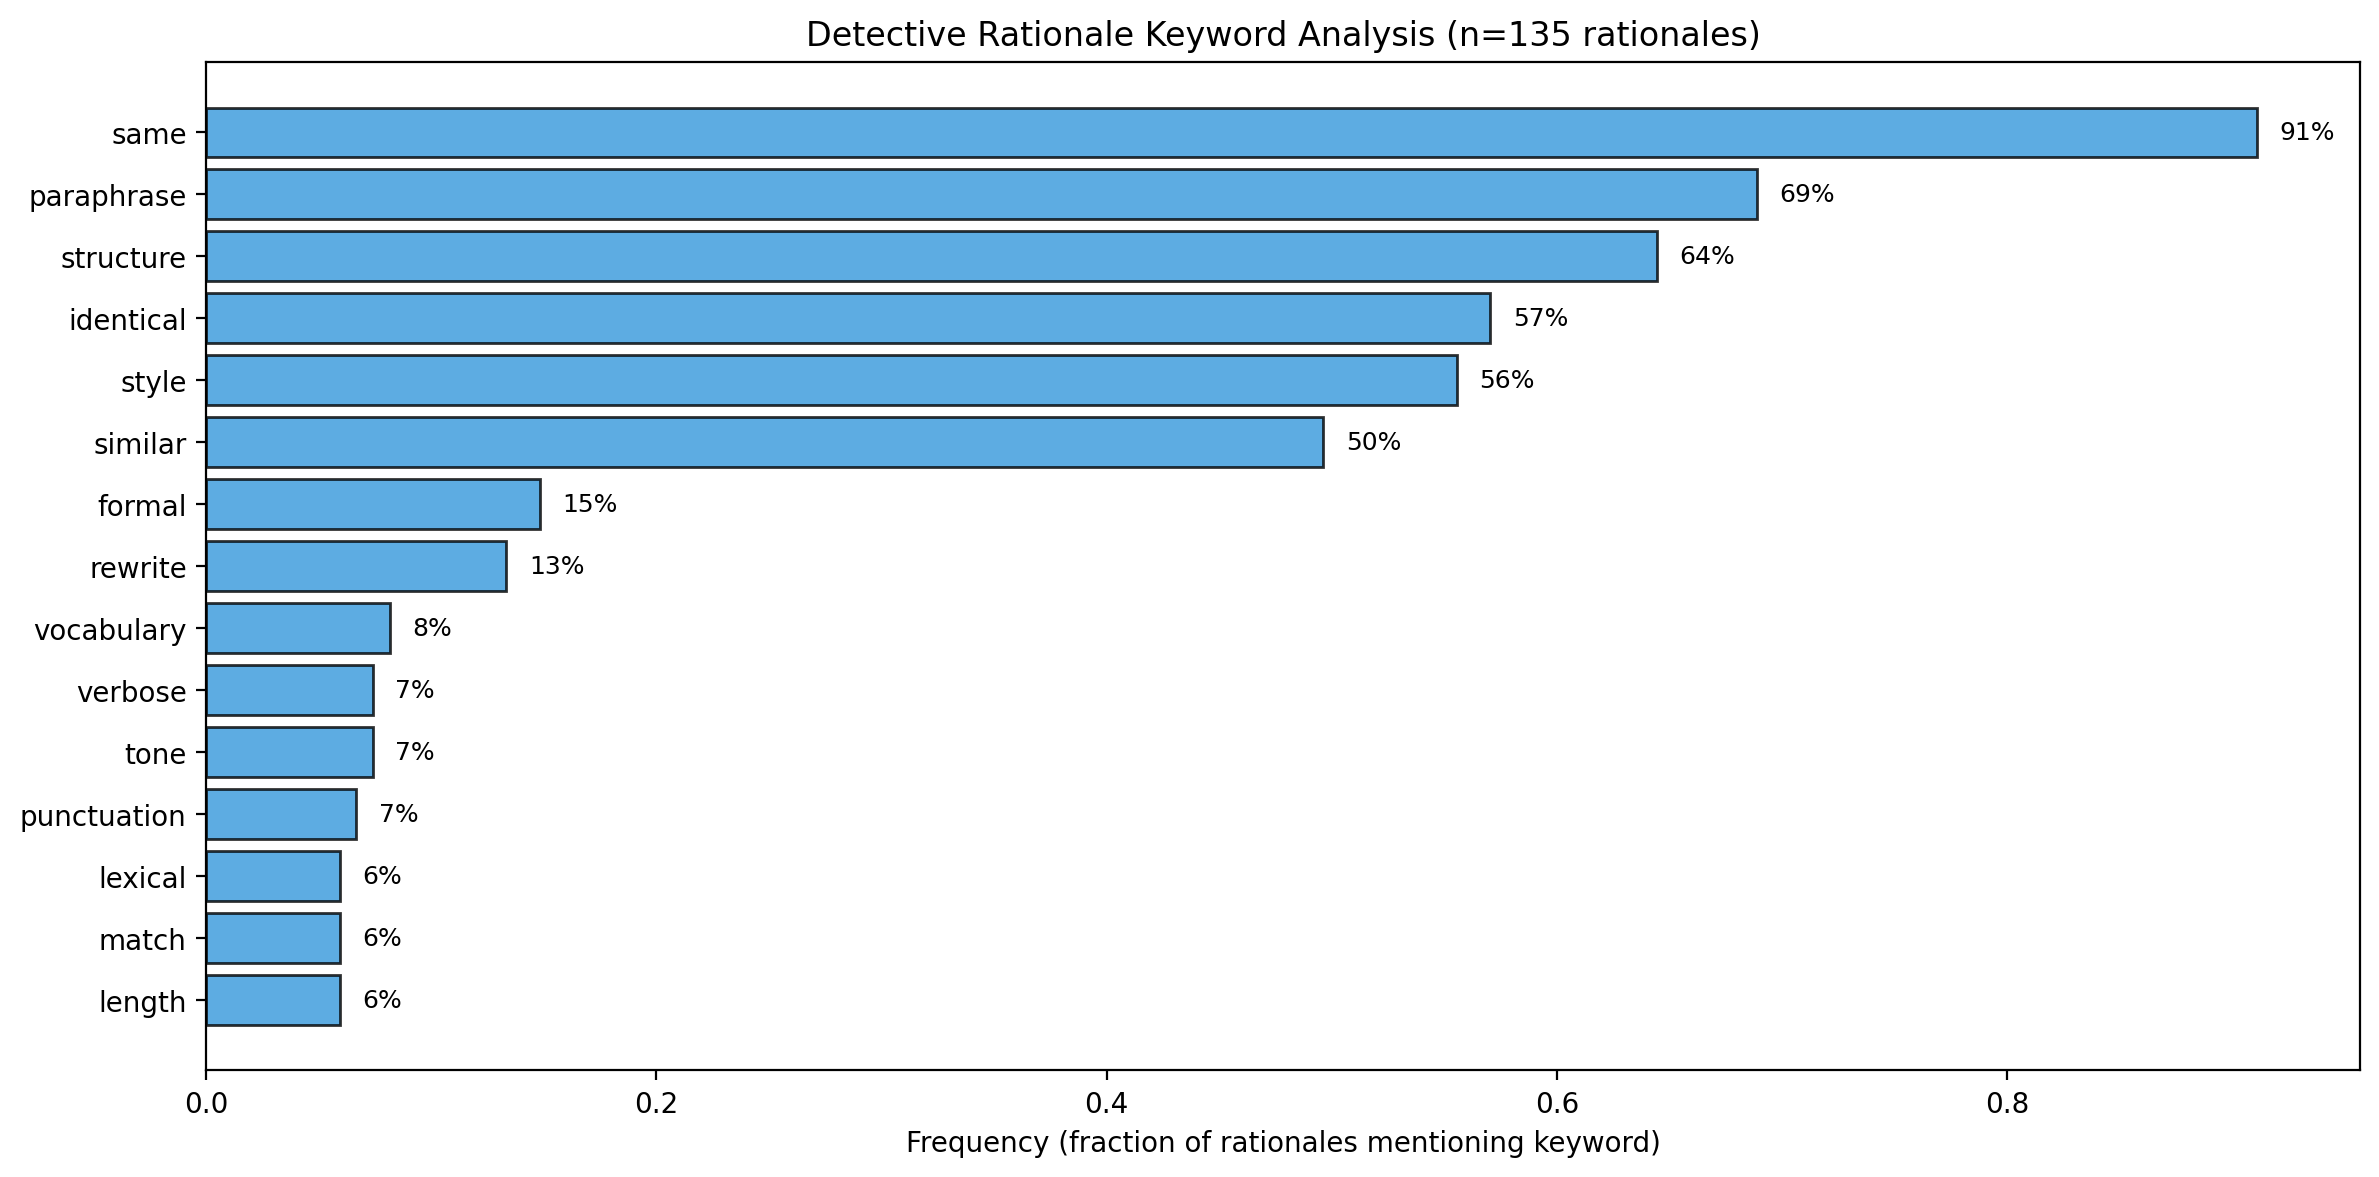
\includegraphics[width=\linewidth]{figures/fig8_rationale_keywords.png}
    \end{column}
    \begin{column}{0.42\textwidth}
      Top features ($n=135$ rationales):
      \begin{itemize}
        \item \textbf{Structure}: 64\%
        \item \textbf{Style}: 56\%
        \item Formal: 15\%
        \item Vocabulary: 8\%
        \item Tone: 7\%
        \item Length: 6\%
      \end{itemize}
      \vspace{0.3em}
      \small Structural/stylistic features dominate over surface heuristics.
    \end{column}
  \end{columns}
\end{frame}

% ── Next Steps ────────────────────────────────────────────────────────────────
\begin{frame}{Next Steps}
  \begin{enumerate}
    \item \textbf{Stronger models} --- Test Claude Opus / GPT-5 as Detective/Auditor
    \item \textbf{Expand paraphraser pool} --- Mistral, Command-R, Qwen; same-family comparisons (Llama-8B vs.\ 70B)
  \end{enumerate}
\end{frame}

% ── Conclusion ────────────────────────────────────────────────────────────────
\begin{frame}{Conclusion}
  \begin{itemize}
    \item Mean detection: \textbf{60.7\%} vs.\ 10\% random baseline ($p<0.001$)
    \item Fingerprint strength varies widely: GPT-5-Nano (100\%) \textrightarrow\ Llama (25\%)
    \item Detective relies on \textbf{structure \& style}, not just output length
    \item APE-generated source texts match hand-crafted trap effectiveness
  \end{itemize}
  \vspace{1em}
  \begin{block}{Takeaway}
    The ``wood grain'' of AI models is real and measurable---paraphraser attribution is feasible.
  \end{block}
\end{frame}

\end{document}
